%
% teil2.tex -- Beispiel-File für teil2 
%
% (c) 2020 Prof Dr Andreas Müller, Hochschule Rapperswil
%
% !TEX root = ../../buch.tex
% !TEX encoding = UTF-8
%
\section{Richardsons Ansatz \label{geostrophisch:section:richardsonAnsatz}}
\kopfrechts{Teil 2}

Richardson wählte einen innovativen, aber im Grunde sehr simplen Ansatz:  
Statt vereinfachter Modelle verwendete er ein vollständiges System bestehend aus vier Differentialgleichungen.
Die erste Gleichung:
\begin{equation}
	\frac{D\vec{v}}{Dt} + 2\vec{\Omega} \times \vec{v} = -\frac{1}{\rho}\nabla p + \vec{g} \\,
	\label{eq:navstok}
\end{equation}
ist eine Form der Navier-Stokes-Gleichung für rotierende Bezugssysteme.
Sie beschreibt die Beschleunigung von Luftmassen, sowie werden darin die Corioliskraft und Druckgradienten berücksichtigt.
Als nächstes verwendete er die Kontinuitätsgleichung:
\begin{equation}
	\frac{\partial \rho}{\partial t} + \nabla \cdot (\rho \vec{v}) = 0 \\,
	\label{eq:kont}
\end{equation}
welche die Massenerhaltung beschreibt.
Also in anderen Worten die Luft kann nicht verschwinden oder aus dem nichts Auftauchen. 
Zudem brauchte er noch eine Gleichung welche die Energie beschreibt, dazu diente 
\begin{equation}
	\frac{Ds}{Dt} = Q \\.
	\label{eq:enrgy}
\end{equation}
Damit werden Temperatur Änderungen durch Transport sowie Expansion und Kompression der Luftmassen ausgedrückt.
Als letztes verwendete er noch das ideale Gasgesetz:
\begin{equation}
	p = \rho R T,
	\label{eq:gasgesetz}
\end{equation}
dieses ist die Physikalische Verbindung von Druck, Temperatur und Dichte eines Gases.  

Er konstruierte eine Schachbrettartiges Gitter und legte es über die Karte von Europa.
Siehe Abbildung~\ref{bild:karteEuropa} dies ist Richardsons Karte mit dem Gitter. 

Nun wollte er für jeden dieser Gitterpunkte das beschriebene Gleichungssystem numerisch von Hand lösen. 

\begin{figure}
	\centering
	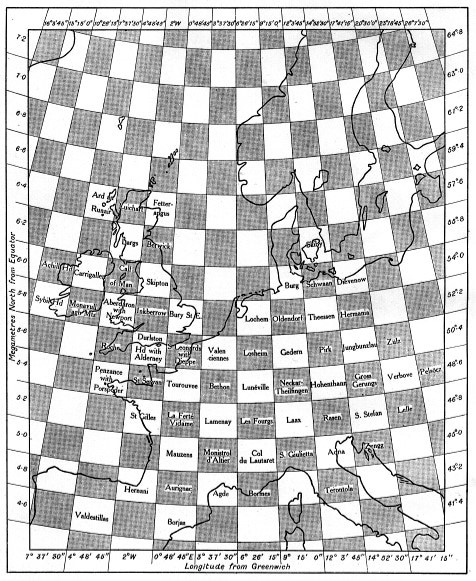
\includegraphics{eingeteilte_Karte.jpg}
	\caption{ll}
	\label{bild:karteEuropa}
\end{figure}



